% BEGIN PREAMBEL
\documentclass[9pt]{beamer}
\usepackage[british]{babel}
\usepackage[latin1]{inputenc}
\usepackage{amsmath,amsfonts,amssymb}
\usepackage{upgreek}
\usepackage{pgfpages}
\usepackage[version=3]{mhchem}
\usepackage{lmodern}
\usepackage{graphicx}
\usepackage{multicol}
\usepackage{xcolor}
\usepackage{wrapfig}
\newcommand{\as}{\\[14pt]}
\newcommand{\s}{\\[7pt]}
\newcommand{\is}{\\[2pt]}
\newcommand{\no}{\noindent}
\newcommand{\ka}{\hspace*{0.5cm}}
\newcommand{\ma}{\hspace*{1cm}}
\newcommand{\ga}{\hspace*{1.5cm}}
\newcommand{\li}{\left|}
\newcommand{\re}{\right|}
\newcommand{\const}{\text{const.}}
\newcommand{\z}{\text}
\newcommand{\terminal}[1]{\colorbox{black}{\textcolor{white}{{\fontfamily{phv}\selectfont \scriptsize{#1}}}}}
\newcommand{\plugin}[1]{\textit{\flq#1\frq}}
\usetheme{Boadilla}
\usecolortheme{beaver}
\useoutertheme{miniframes}
\beamertemplatenavigationsymbolsempty
\makeindex
\title[Pixel Detectors]{Preliminary Results of Pixel Detectors in 2015 PSI Testbeams}
\author[M. Reichmann]{Michael Reichmann}
\institute[\textbf{\textit{ETH}}\scalebox{.6}{\textit{Z\"{u}rich}}]{Swiss Federal Institute of Technology Zurich}
% END PREAMBEL
\begin{document}
% ============================
% TITLE PAGE
% ============================
\begin{frame}
	\begin{center}
		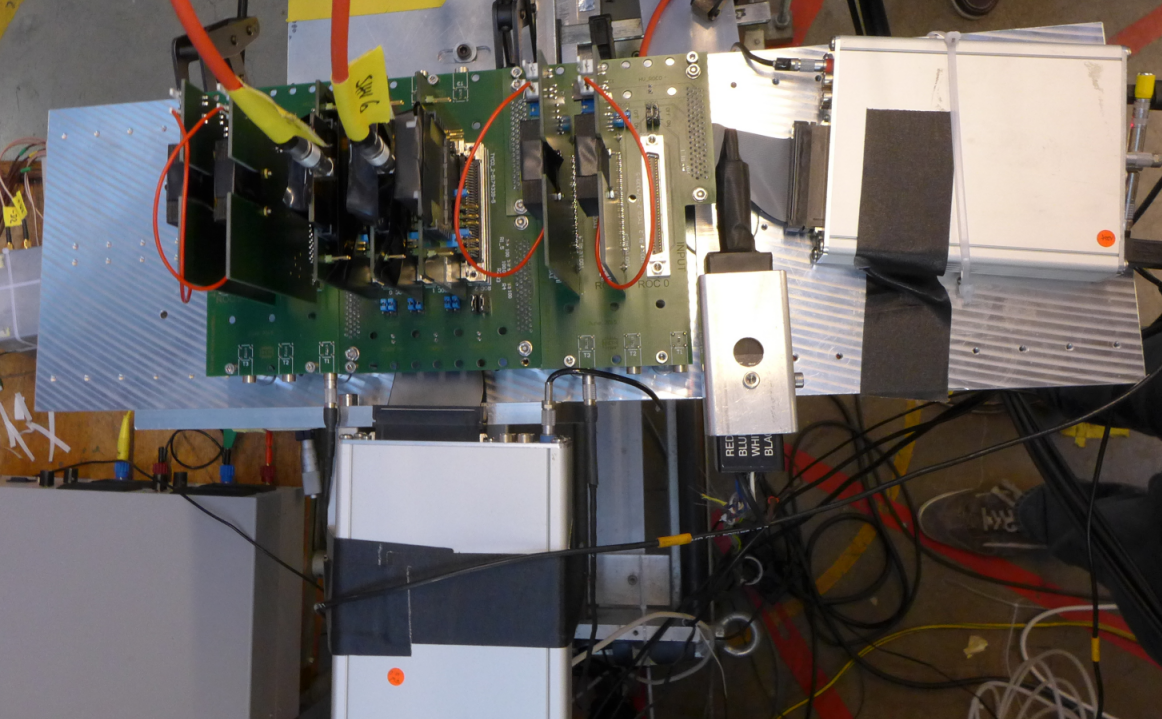
\includegraphics[width=8cm]{Pics/setupfull}
	\end{center}
	\begin{alertblock}{
		\begin{center}
			\textbf{Preliminary Results of Pixel Detectors in 2015 PSI Testbeams}
		\end{center}}
		\vspace*{10pt}
		\begin{center}\small
		Michael Reichmann
		\end{center}\normalsize
	\end{alertblock}
\end{frame}
% ============================
% TABLE OF CONTENTS
% ============================
\begin{frame}%[allowframebreaks]
	\frametitle{Table of contents}
	\tableofcontents   % [pausesections]
\end{frame}
% ====================================================================================
% TELESCOPE
% ====================================================================================
\section{The Telescope}
\begin{frame}
	\begin{alertblock}{
		\begin{center}
			\Large{\textbf{The Telescope}}
		\end{center}}
	\end{alertblock}
\end{frame}
% ============================
% GENERAL SETUP
\subsection{General Setup}
\begin{frame}
	\frametitle{General Setup}
	\begin{center}
		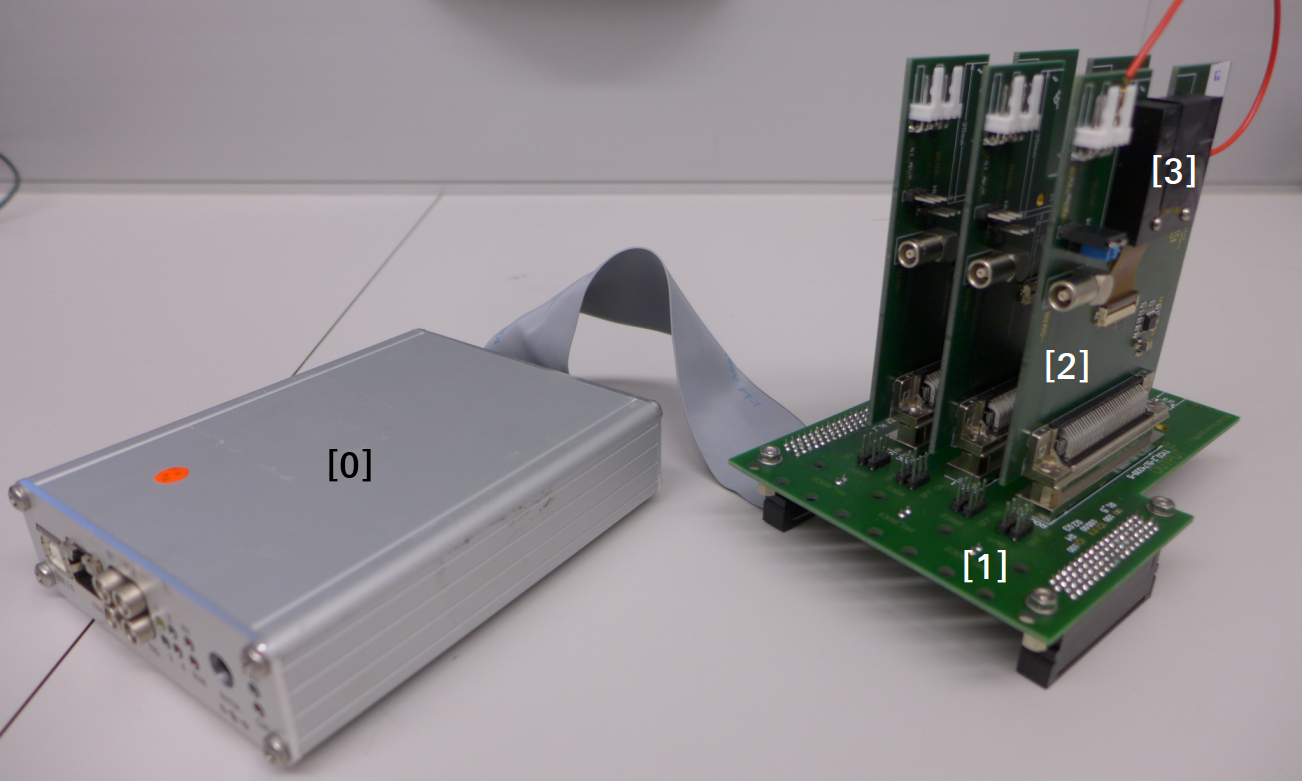
\includegraphics[width=6cm]{Pics/setup}
	\end{center}
	\begin{itemize}
		\item $[0]$ DTB (Digital Test Board) as interface between telescope and computer
		\item $[1]$ Motherboard as main frame for the telescope
		\item $[2]$ Adapter Planes as mounting framework for the single pixel chips
		\item $[3]$ CMS Pixel Chip (analogue or digital)
	\end{itemize}
\end{frame}
% ============================
% MOTHERBOARD
\subsection{Motherboard}
\begin{frame}
	\frametitle{Motherboard}
	\begin{center}
		\begin{minipage}{4.5cm}
			\centering
			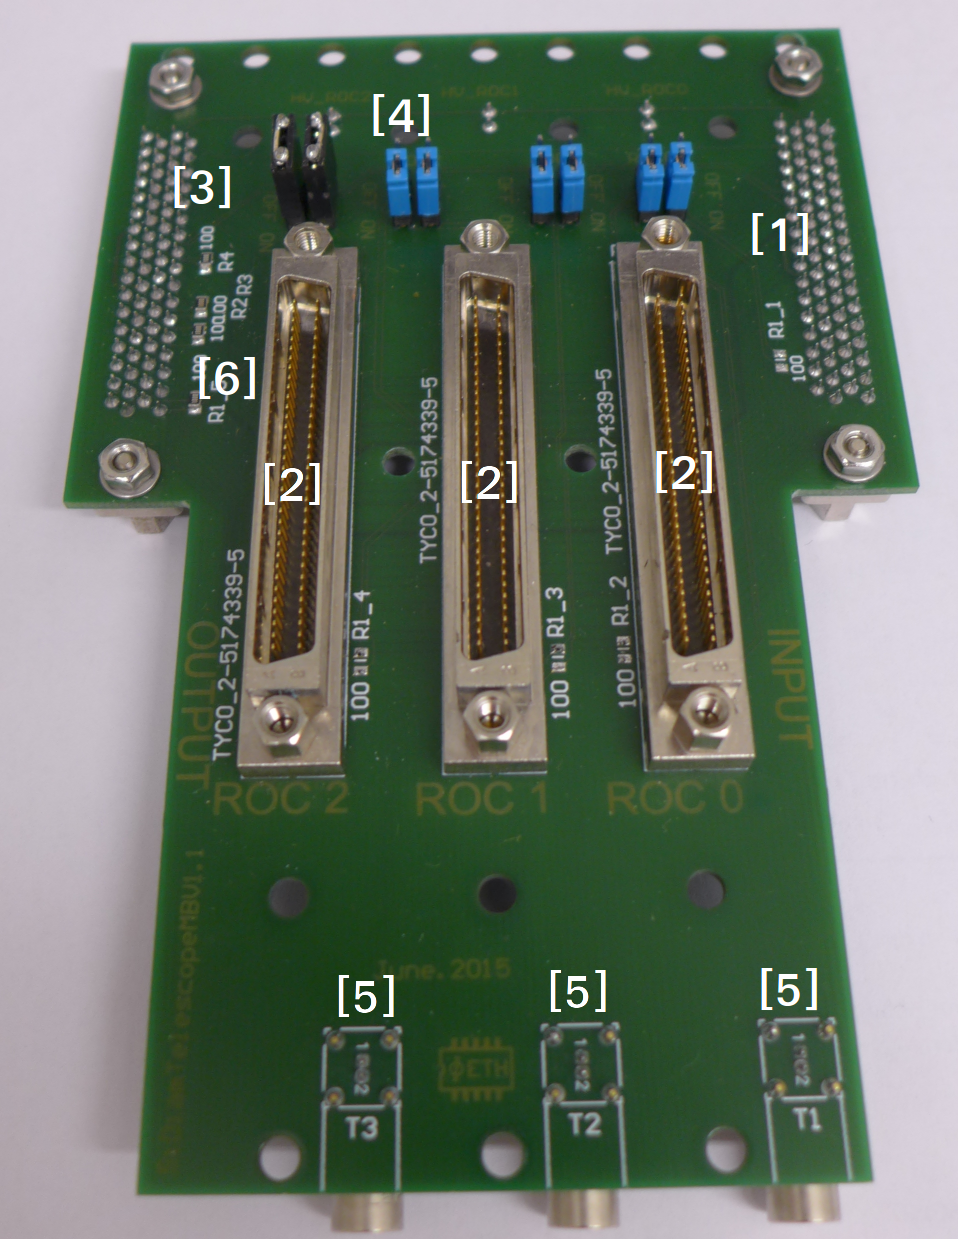
\includegraphics[width=4.2cm]{Pics/mb2}
		\end{minipage}
		\hspace*{2pt}
		\begin{minipage}{6cm}
			\begin{itemize}
				\item $[1]$ input scsi connector to the DTB
				\item $[2]$ sockets for the adapter planes
				\item $[3]$ optional output scsi connector to another motherboard (chainable)
				\item $[4]$ token jumpers (blue: plane active, black: plane inactive) 
				\item $[5]$ LEMO output of the fast-OR trigger signal 
				\item $[6]$ termination of the signals
			\end{itemize}
		\end{minipage}\no\s
	\end{center}
\end{frame}
% ============================
% PLANE
\subsection{Adapter Plane}
\begin{frame}
	\frametitle{Adapter Plane}
	\begin{center}
		\begin{minipage}{4.5cm}
			\centering
			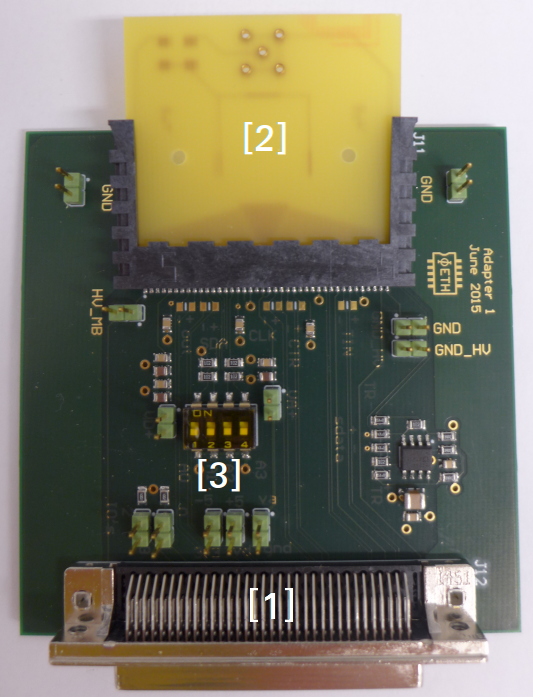
\includegraphics[width=4.2cm]{Pics/digada}
		\end{minipage}
		\hspace*{2pt}
		\begin{minipage}{6cm}
			\begin{itemize}
				\item $[1]$ scsi connector to the motherboard
				\item $[2]$ digital CMS pixel chip on a pcb (back side)
				\item $[3]$ I$^{2}$C address bit switch
			\end{itemize}
		\end{minipage}\no\s
	\end{center}
\end{frame}
% ====================================================================================
% BEGIN PIXEL SETUP
% ====================================================================================
\section{The Pixel Setup}
\begin{frame}
	\begin{alertblock}{
		\begin{center}
			\Large{\textbf{The Pixel Setup}}
		\end{center}}
	\end{alertblock}
\end{frame}
% new frame ==================
\begin{frame}
	\frametitle{Pixel Setup}
	\begin{center}
		\begin{minipage}{4.5cm}
			\centering
			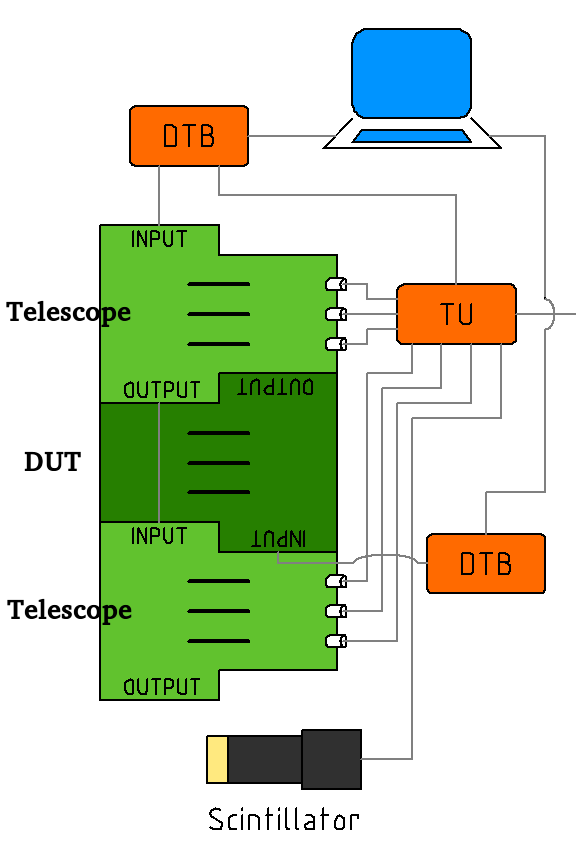
\includegraphics[width=4.0cm]{Pics/fulltel_scint}
		\end{minipage}
		\hspace*{2pt}
		\begin{minipage}{6cm}
			\begin{itemize}
				\item telescope consistant of two chained motherboards with 4 (6) planes and analogue ROCs (Read Out Chips)
				\item DUT consistant of one motherboard with up to three planes with digital pixelated diamond sensors
				\item both read out by seperate DTBs
				\item scintillator for precise timing
				\item fast-OR triggers of the analogue chips and scintillator connected to a TU (Trigger Unit) 
				\item TU sends trigger back to the DTBs
			\end{itemize}
		\end{minipage}\no\s
	\end{center}
\end{frame}
% ============================
% THE DIGITAL TESTBOARD
\subsection{The DTB}
\begin{frame}
	\frametitle{The Digital Test-Board}
	\begin{itemize}
		\item FPGA including soft Token Bit Manager (TBM) emulator
		\item clock and external trigger inputs
		\item connectors: USB, low voltage and scsi 
		\item LEMO high voltage input for biasing the sensors
		\item internal ADC
	\end{itemize}
	\begin{center}
		\begin{minipage}{5cm}
			\centering
			\begin{figure}
				\caption{DTB inside}
				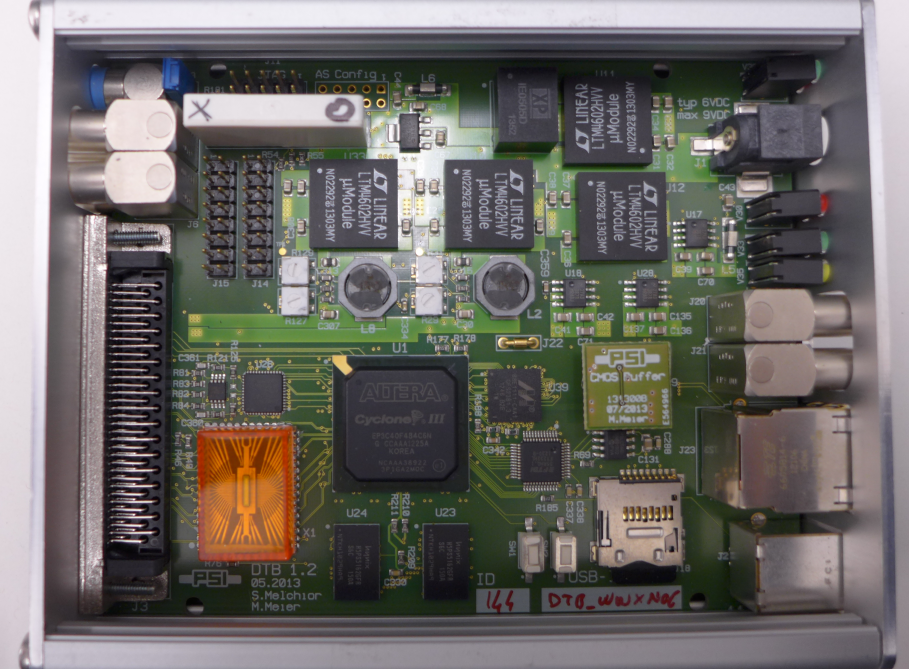
\includegraphics[width=4.5cm]{Pics/dtb_inside}
			\end{figure}
		\end{minipage}
		\hspace*{2pt}
		\begin{minipage}{5cm}
			\centering
			\begin{figure}
				\caption{DTB front and back}
				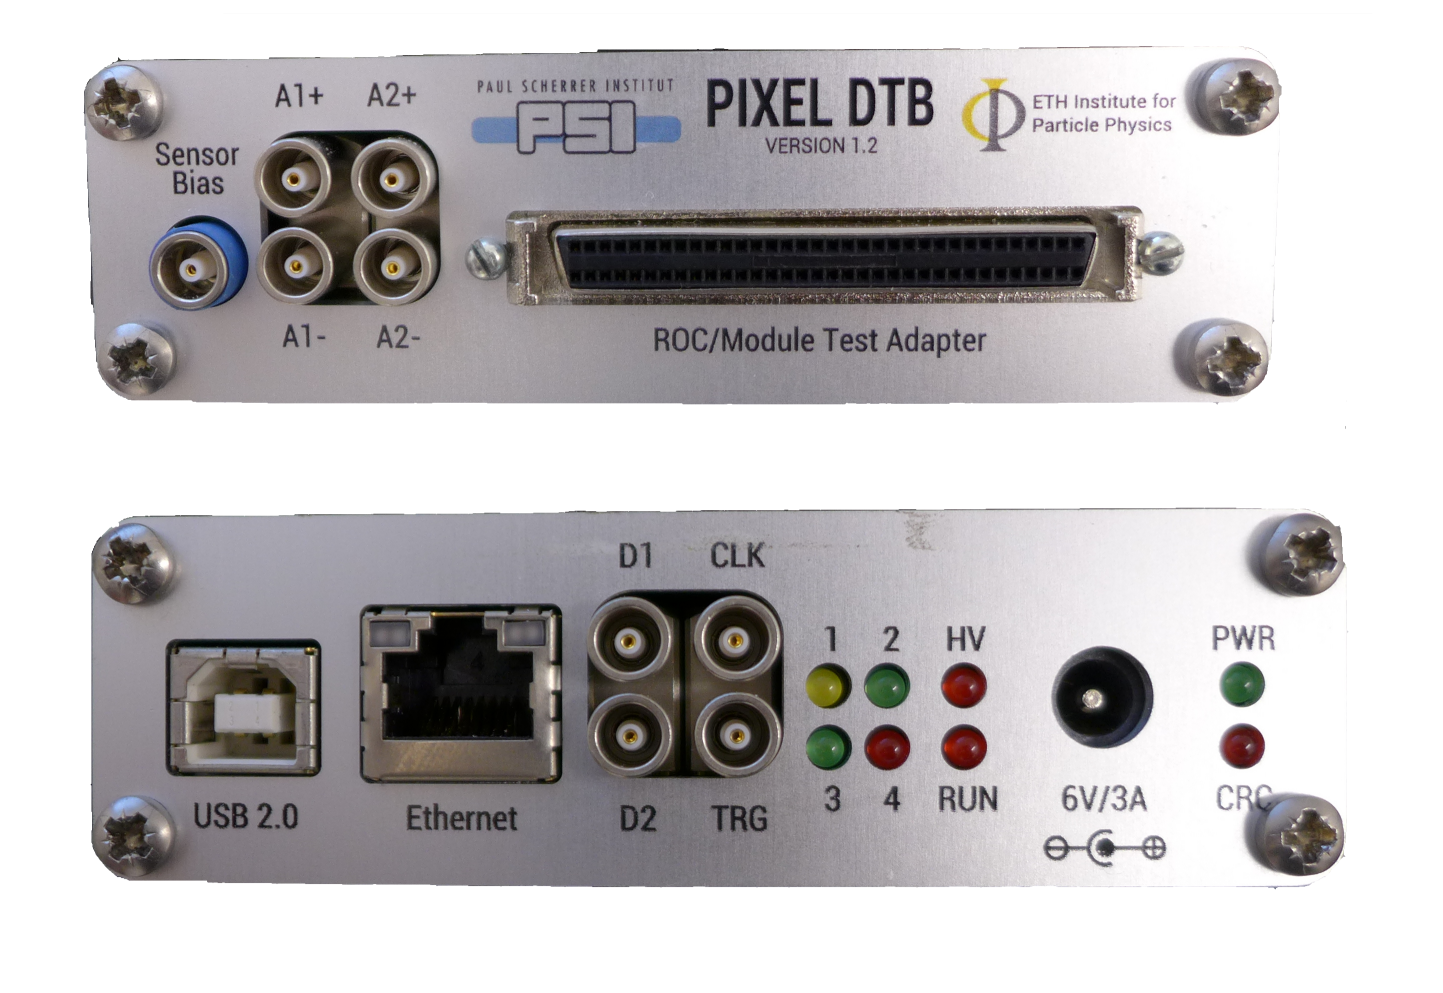
\includegraphics[width=4.5cm]{Pics/DTB-Sides}
			\end{figure}
		\end{minipage}\no\s
	\end{center}
\end{frame}
% ============================
% PIXEL SETUP
\subsection{Trigger Logic}
\begin{frame}
	\frametitle{Trigger Logic}
	\begin{center}
		\begin{minipage}{6cm}
			\centering
			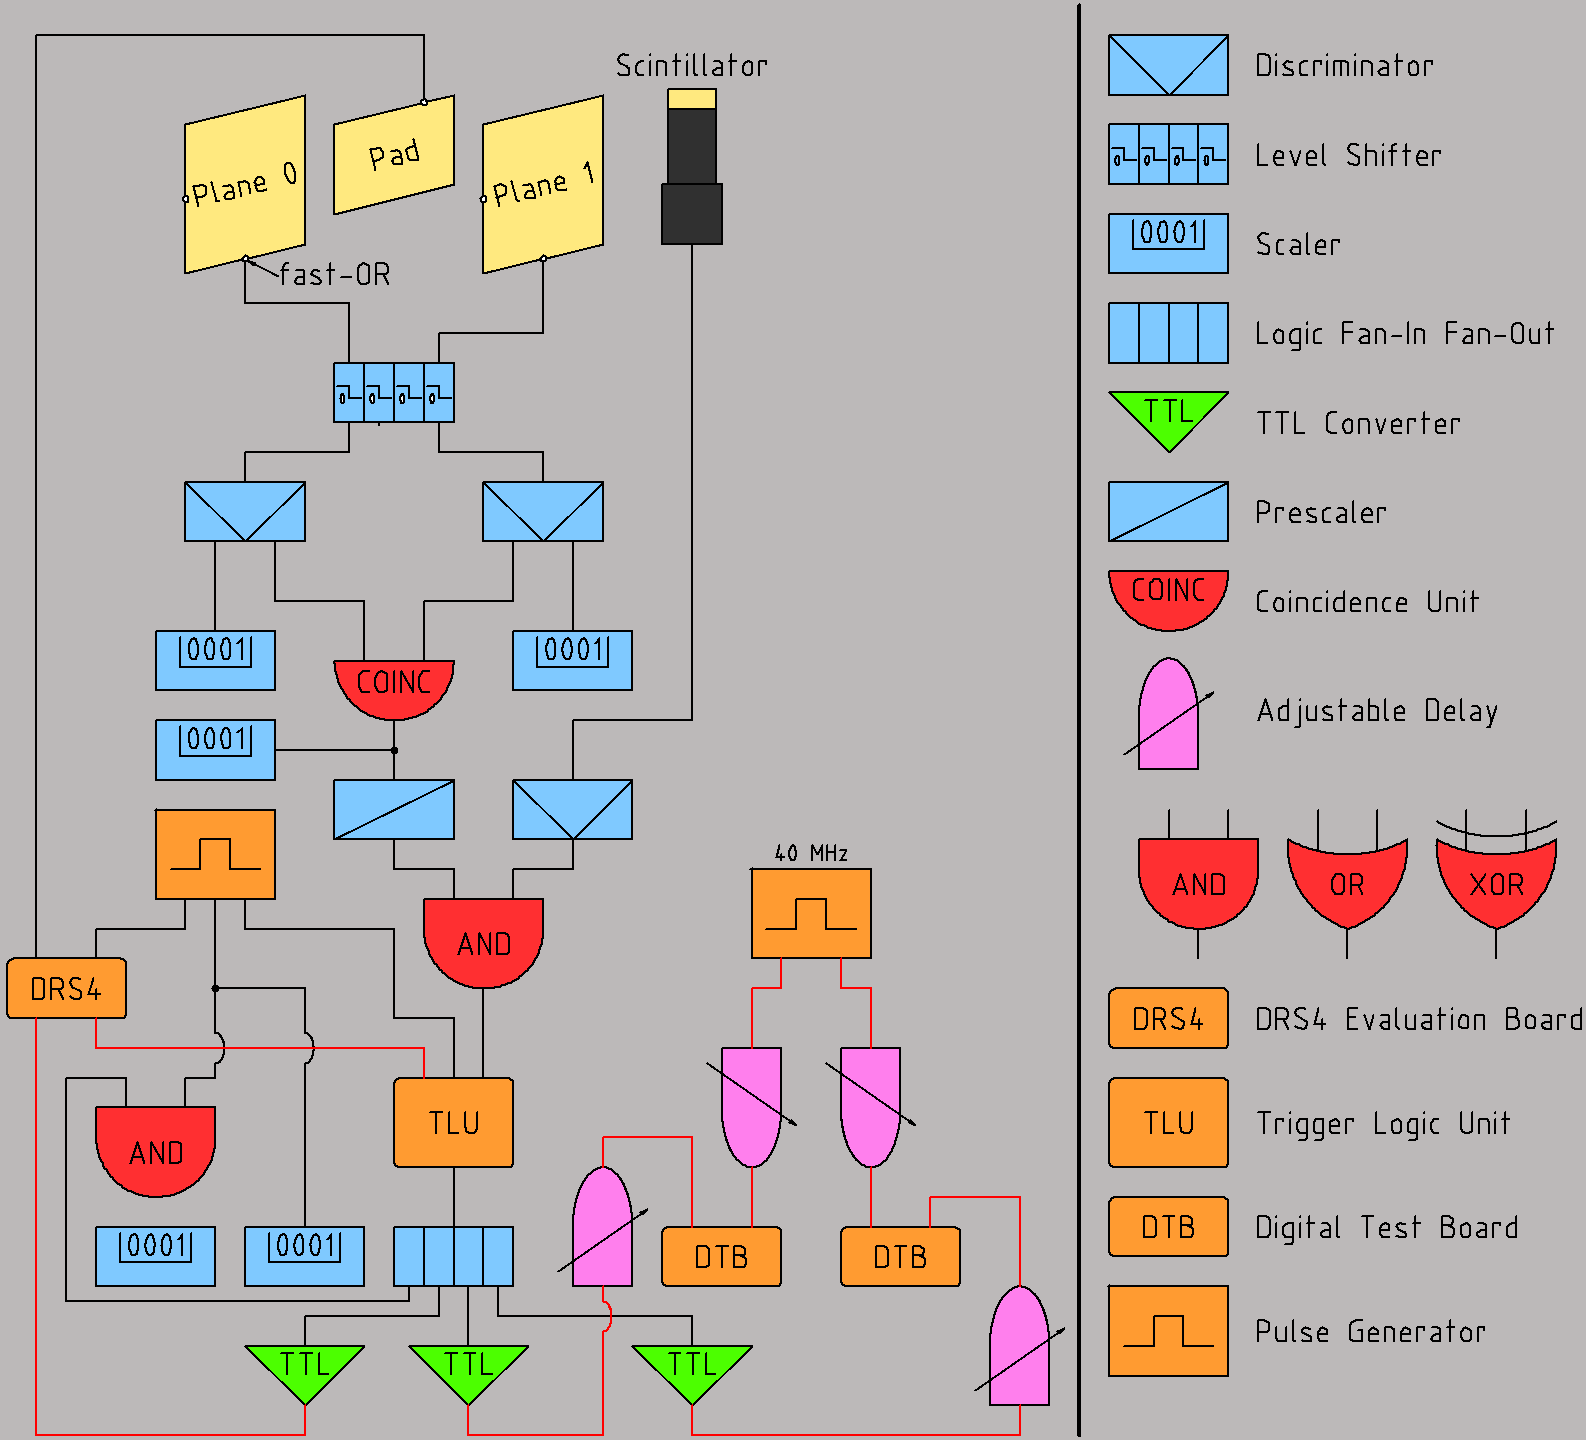
\includegraphics[width=6cm]{Pics/triglog2}
		\end{minipage}
		\hspace*{2pt}
		\begin{minipage}{5cm}
			\begin{itemize}
				\item coincidence between a fast-OR of planes before and after the DUT
				\item AND of scintillator and fast-OR coincidence as trigger
				\item trigger has adjustable delays for both telescopes
				\item global external clock with adjustable delays for pixel telescope
				\item generated busy signal after trigger to avoid event misalignment
				\begin{itemize}
					\item useful for long events with many pixels hit 
				\end{itemize}
			\end{itemize}
		\end{minipage}\no\s
	\end{center}
\end{frame}
% END PIXEL SETUP
% ====================================================================================
% DATATAKING
% ====================================================================================
\section{The Datataking}
\begin{frame}
	\begin{alertblock}{
		\begin{center}
			\Large{\textbf{The Datataking}}
		\end{center}}
	\end{alertblock}
\end{frame}
% ============================
% pXar
\subsection{pXar}
\begin{frame}
	\frametitle{pXar}
	\begin{center}
		
\includegraphics[width=3cm]{Pics/pxar_logo}
	\end{center}
	\begin{itemize}
		\item short for Pixel eXpert Analysis Readout
		\item software for communication between the telescope and a computer
		\item pXar-core libraries: program and readout information of the the CMS pixel chips
		\item python CLI (Command Line Interface) to perform simple tests
	\end{itemize}
\end{frame}
% ============================
% EUDAQ
\subsection{EUDAQ}
\begin{frame}
	\frametitle{EUDAQ}
% 	\begin{center}
% 		\begin{minipage}{4.5cm}
% 			\centering
% 			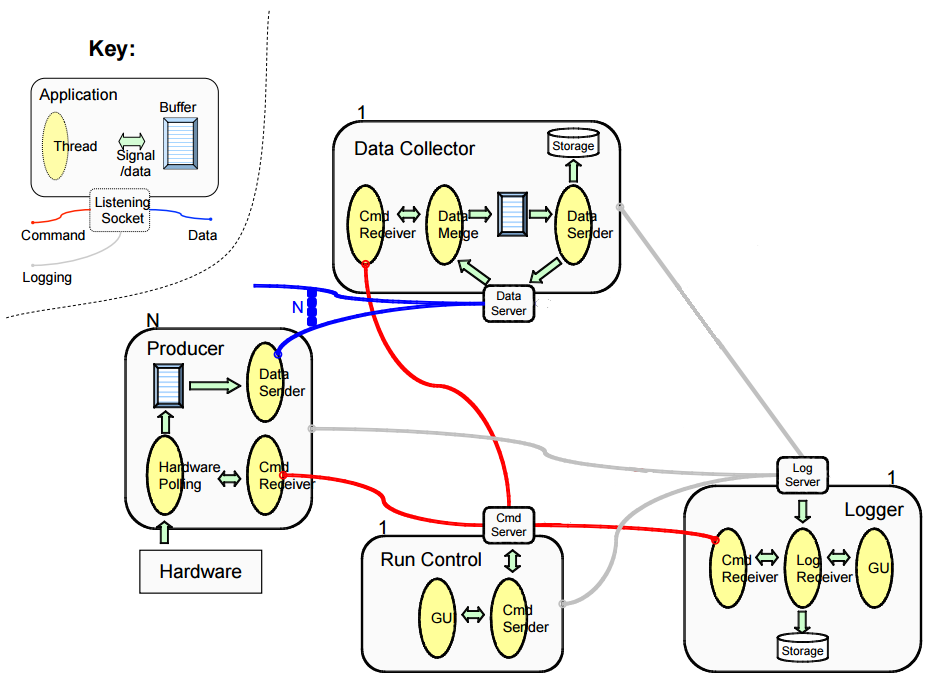
\includegraphics[width=4.2cm]{Pics/eudaq}
% 		\end{minipage}
% 		\hspace*{2pt}
% 		\begin{minipage}{6cm}
			\begin{itemize}
				\item portable, modular and cross-platform DAQ framework
				\item developed for the EUDET Pixel Telescope
				\item can combine data streams from several different devices into an event based data stream
				\item adapting software to our purposes with help of DESY 
				\item using pXar core libraries
			\end{itemize}
% 		\end{minipage}\no\s
% 	\end{center}
\end{frame}
% ============================
% WBC SCAN
\subsection{WBC scan}
\begin{frame}
	\frametitle{WBC scan}
	\begin{center}
		\begin{minipage}{4.0cm}
			\centering
			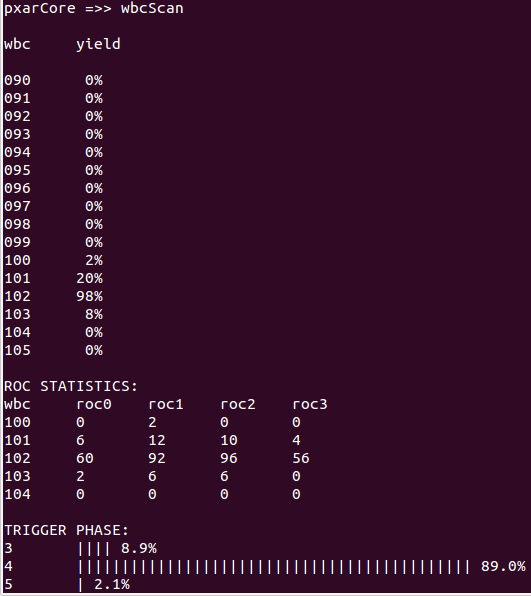
\includegraphics[width=4.0cm]{Pics/wbcscan1}
		\end{minipage}
		\hspace*{2pt}
		\begin{minipage}{7cm}
			\begin{itemize}
				\item ROC saves bunch crossing when particle hits the sensor
				\item programmable setting called wbc (wait bunch crossing)
				\item trigger only validates if time the trigger takes back to the ROC matches the wbc setting
				\item automated wbc scan using the pXar CLI
				\item detailed information about the hit yield (event has at least one hit) for every connected ROC
				\item information of the trigger phase (relative timing of the trigger compared to the clock)
			\end{itemize}
		\end{minipage}\no\s
	\end{center}
\end{frame}
% ============================
% OPTIMISATION
\subsection{Efficiency Optimisation}
\begin{frame}
	\frametitle{Telescope}
	\begin{itemize}
		\item fast-Or trigger sampled with 25ns clock $\rightarrow$ jitters within 25ns window
		\item coincidence with scintillator splits up trigger phase
		\item use trigger delay to shift the trigger into the place within the clock so that efficiency is maximised
	\end{itemize}
\end{frame}
% new frame ==================
\begin{frame}
	\frametitle{DUT}
	\begin{center}
		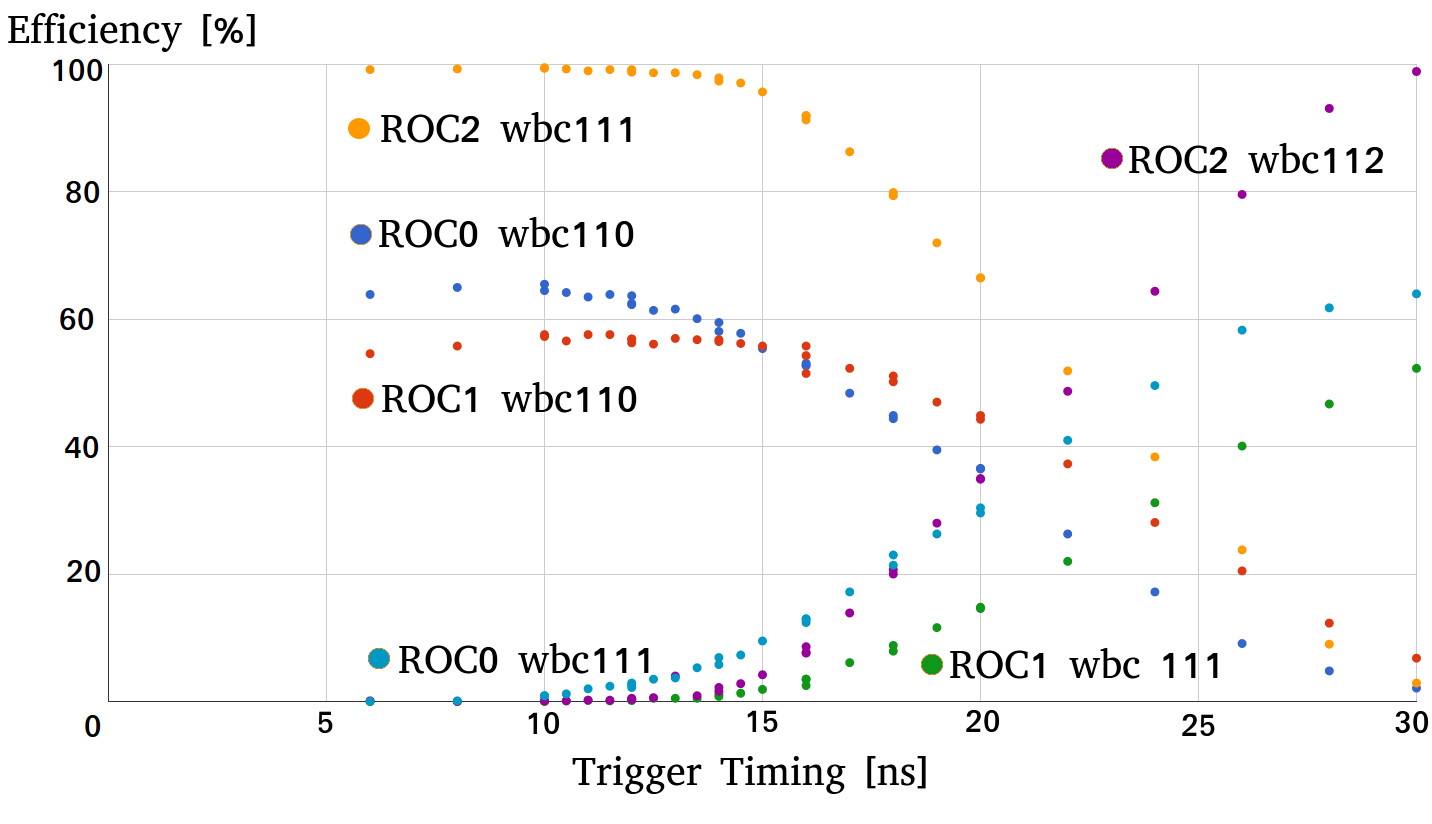
\includegraphics[height=4.5cm]{Pics/optimisation}
	\end{center}
	\begin{itemize}
		\item first use trigger delay to shift the the trigger in the middle of the clock
		\item shift trigger and clock delay together
		\begin{itemize}
			\item leaves trigger phase constant
			\item find optimal efficiency relative to the telescope clock
		\end{itemize}

	\end{itemize}
\end{frame}
% ============================
% CURRENTS
\subsection{Current Monitor}
\begin{frame}
	\frametitle{Current Monitor}
	\begin{center}
		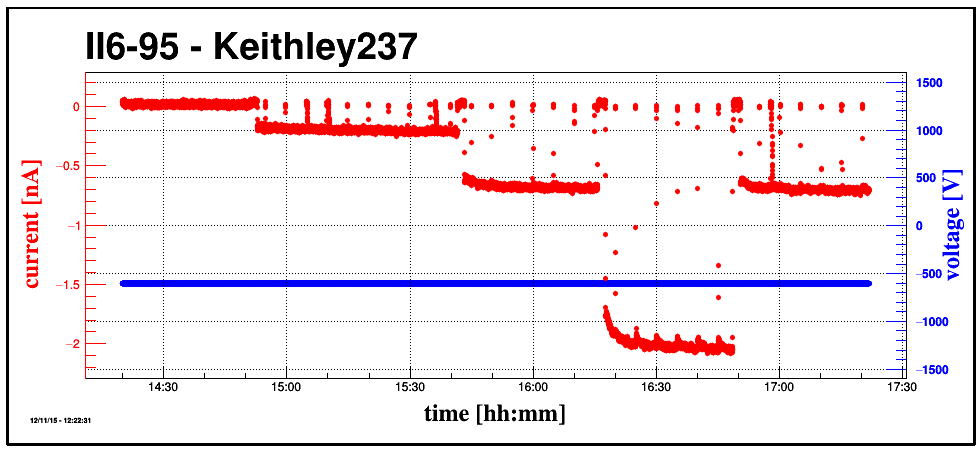
\includegraphics[height=4cm]{Pics/currents}
	\end{center}
	\begin{itemize}
		\item monitoring of the currents of the diamonds during the whole beam test
		\item beam induced currents for higher rates
		\item current drops to 0 at beam interruptions
	\end{itemize}
\end{frame}
% ====================================================================================
% MEASUREMENTS
% ====================================================================================
\section{The Measurements}
\begin{frame}
	\begin{alertblock}{
		\begin{center}
			\Large{\textbf{The Measurements}}
		\end{center}}
	\end{alertblock}
\end{frame}
% new frame ==================
\begin{frame}
	\frametitle{Types of Measurements}
	\begin{itemize}
		\item two beam tests at PSI
		\item tested diamonds unirradiated:
			\begin{itemize}
				\item II6-94, II6-95
			\end{itemize}
		\item tested diamonds irradiated:
			\begin{itemize}
				\item II6-95
			\end{itemize}
		\item beam rate scans (up$\rightarrow$down$\rightarrow$up)
		\item different bias voltages
		\item closing beam shutter before the run was startet and open it during the begin of the run
		\item not closing the beam shutter
		\item experimental runs:
		\begin{itemize}
			\item continuously changing the particle rate during the run
			\item continuously changing the bias voltage during the run
			\item very low ROC threshold (noisy chip)
		\end{itemize}
	\end{itemize}
\end{frame}
% ====================================================================================
% Analysis
% ====================================================================================
\section{The Analysis}
\begin{frame}
	\begin{alertblock}{
		\begin{center}
			\Large{\textbf{The Analysis}}
		\end{center}}
	\end{alertblock}
	\begin{itemize}
		\item preliminary results
		\item offline analysis has not started yet
		\item online analysis during the beam test with online monitor
		\item pre analysis with tracking software
	\end{itemize}
\end{frame}
% ============================
% ONLINEMON
\subsection{Online Monitor}
\begin{frame}
	\frametitle{Correlations}
	\begin{center}
		\begin{minipage}{5.5cm}
			\centering
			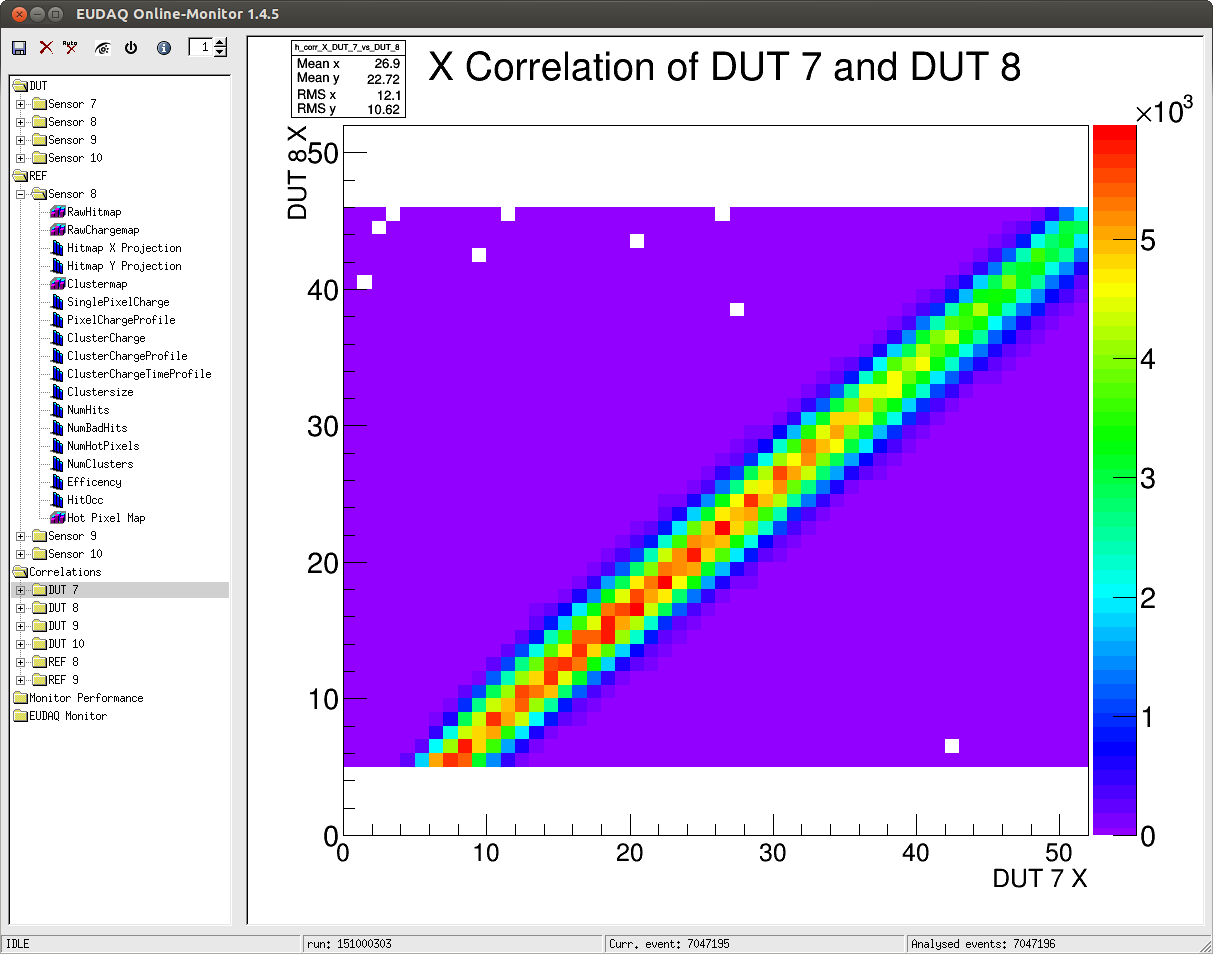
\includegraphics[width=4.0cm]{Pics/correlation1x.png}
		\end{minipage}
		\hspace*{2pt}
		\begin{minipage}{5.5cm}
			\centering
			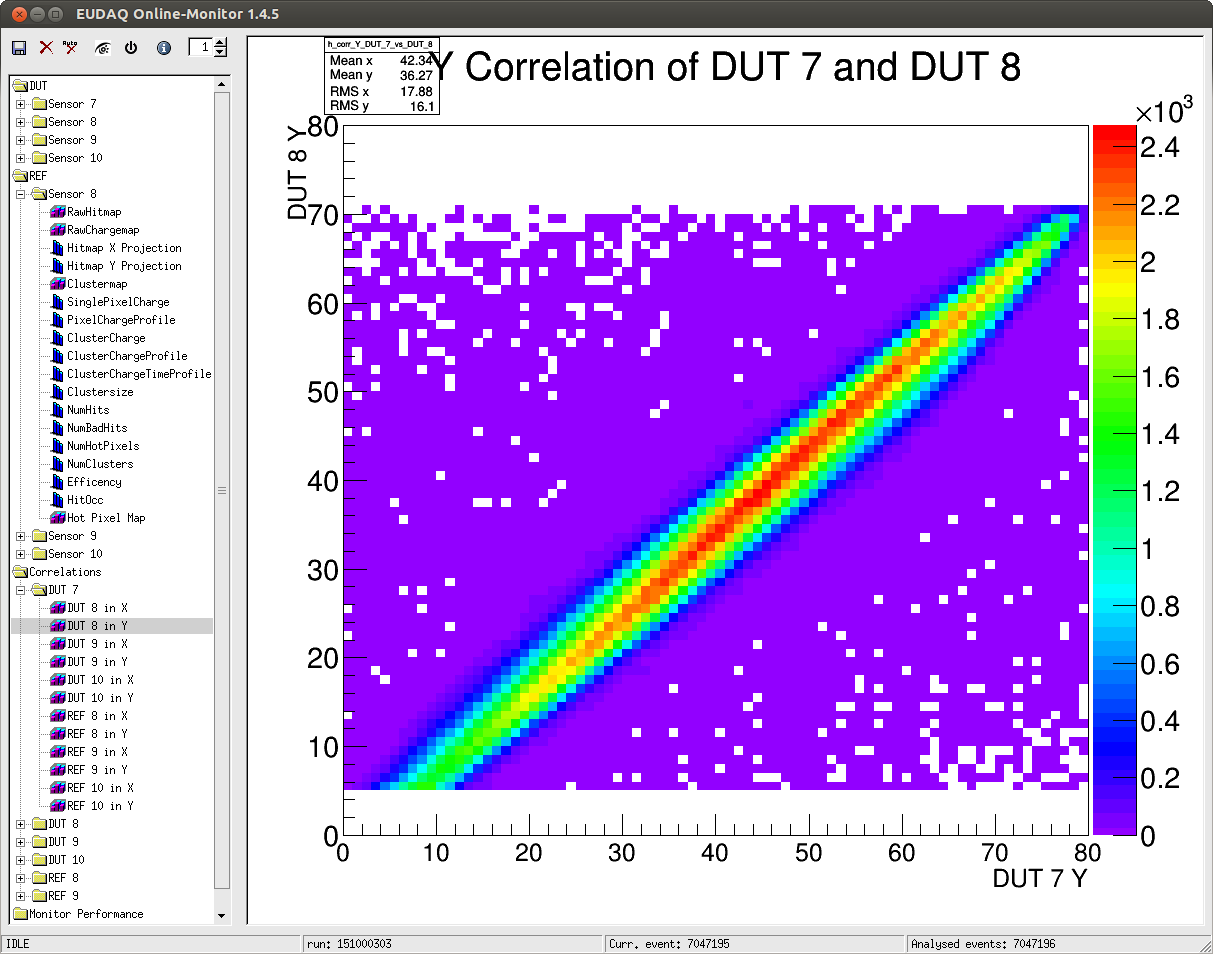
\includegraphics[width=4.0cm]{Pics/correlation1y.png}
		\end{minipage}\no\s
		\begin{minipage}{5.5cm}
			\centering
			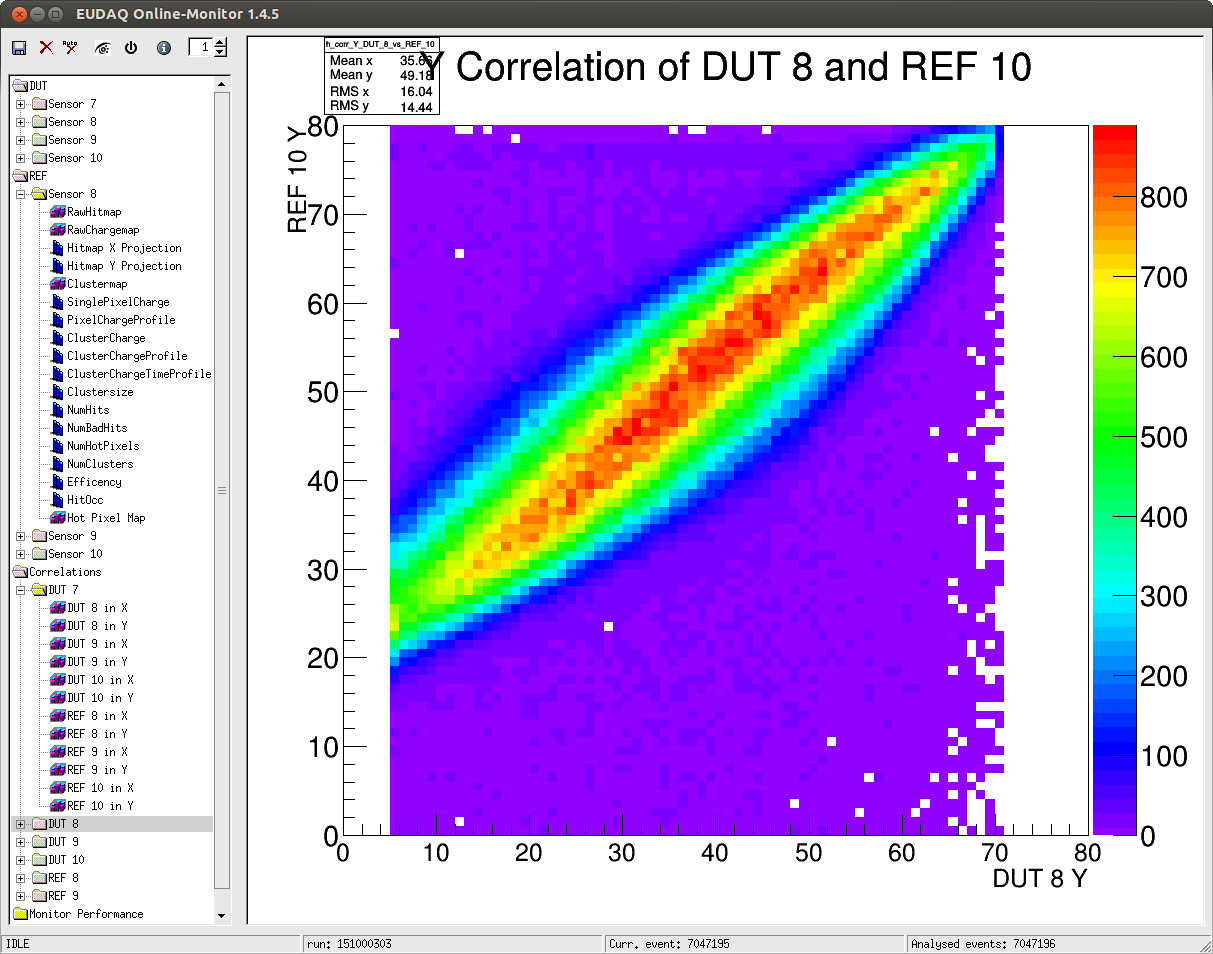
\includegraphics[width=4.0cm]{Pics/correlation2y.png}
		\end{minipage}
		\hspace*{2pt}
		\begin{minipage}{5.5cm}
			\centering
			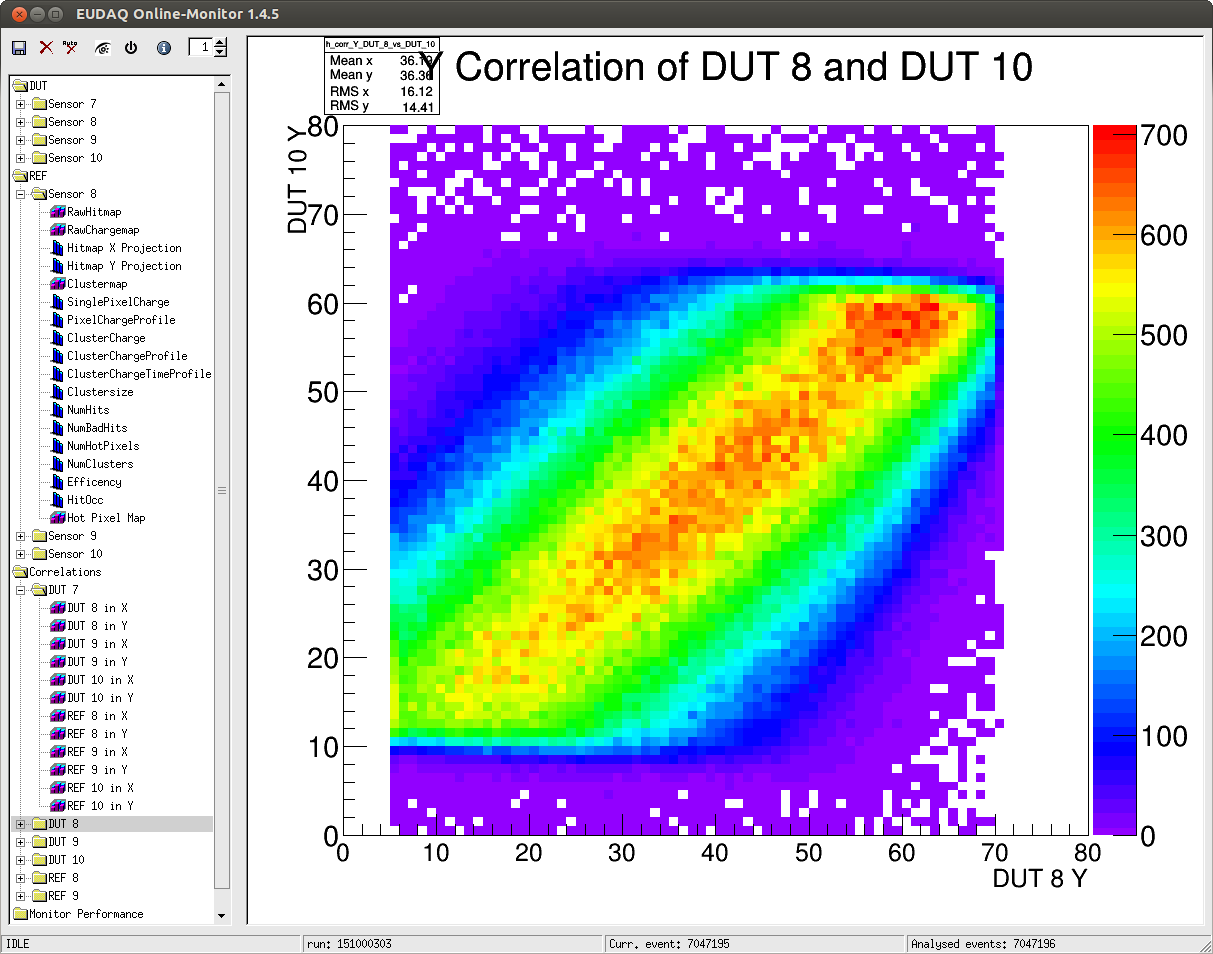
\includegraphics[width=4.0cm]{Pics/correlation3y.png}
		\end{minipage}\no\s
	\end{center}
\end{frame}
% new frame ==================
% \begin{frame}
% 	\frametitle{Signal Distribution}
% 	\begin{itemize}
% 		\item
% 	\end{itemize}
% \end{frame}
% ============================
% TRACKING
\subsection{Tracking}
\begin{frame}
	\frametitle{Pulseheight Distribution}
	\begin{center}
		\begin{minipage}{5.5cm}
			\centering
			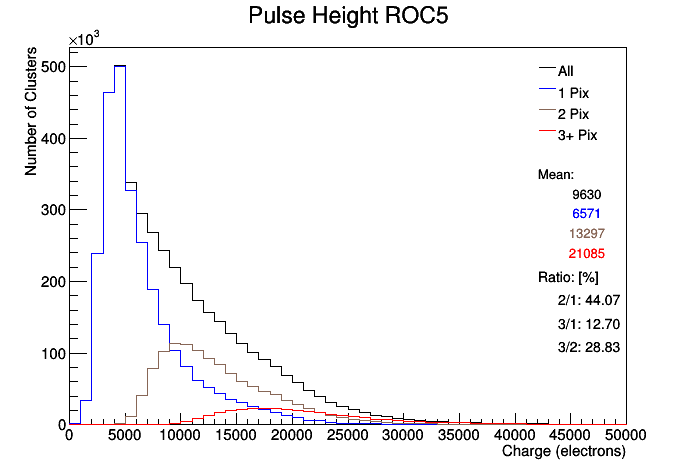
\includegraphics[width=5.5cm]{Pics/PulseHeight_ROC5}
		\end{minipage}
		\hspace*{2pt}
		\begin{minipage}{5.5cm}
			\centering
			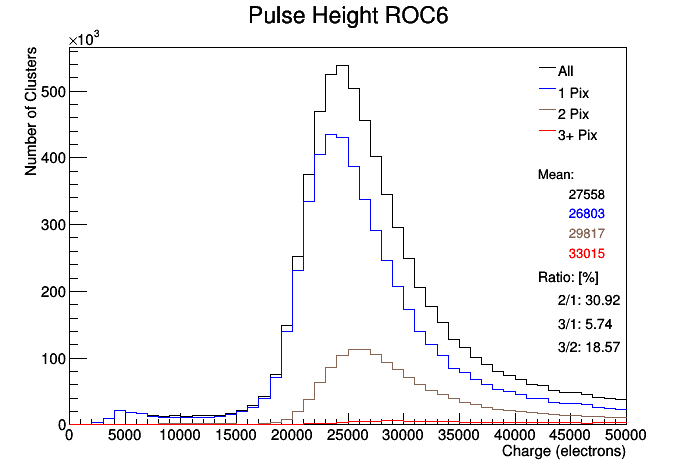
\includegraphics[width=5.5cm]{Pics/PulseHeight_ROC6}
		\end{minipage}\no\s
		\begin{itemize}
		\item ROC5 digital silicon ROC well calibrated with Xray fluorescent lines
		\item ROC6 digital diamond pixel chip, not calibrated
	\end{itemize}
	\end{center}
\end{frame}
% new frame ==========================
\begin{frame}
	\frametitle{Event Display}
	\begin{center}
		\begin{minipage}{5.5cm}
			\centering
			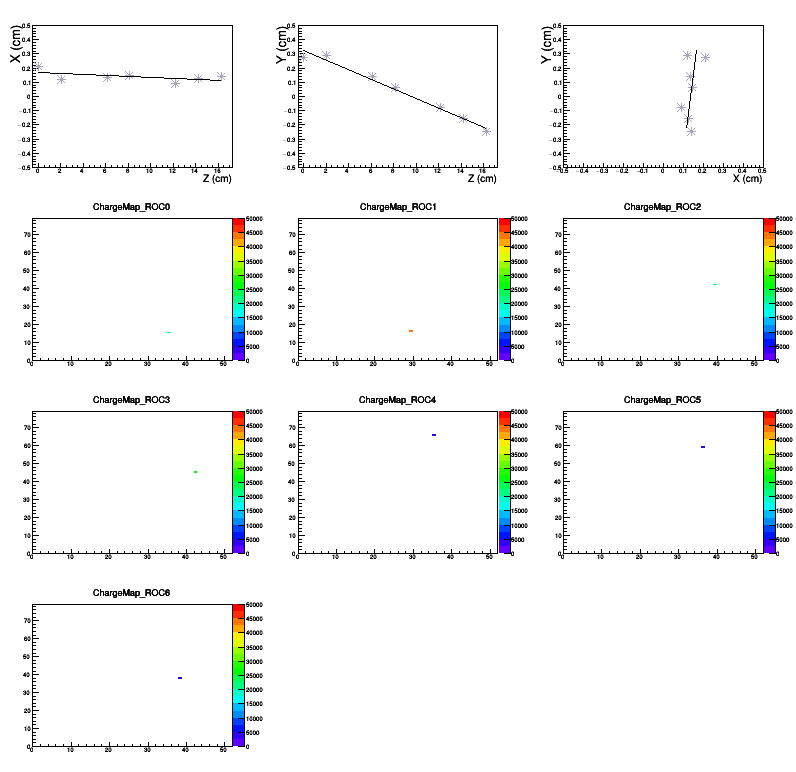
\includegraphics[width=5.5cm]{Pics/Tracks_Ev2}
		\end{minipage}
		\hspace*{2pt}
		\begin{minipage}{5.5cm}
			\centering
			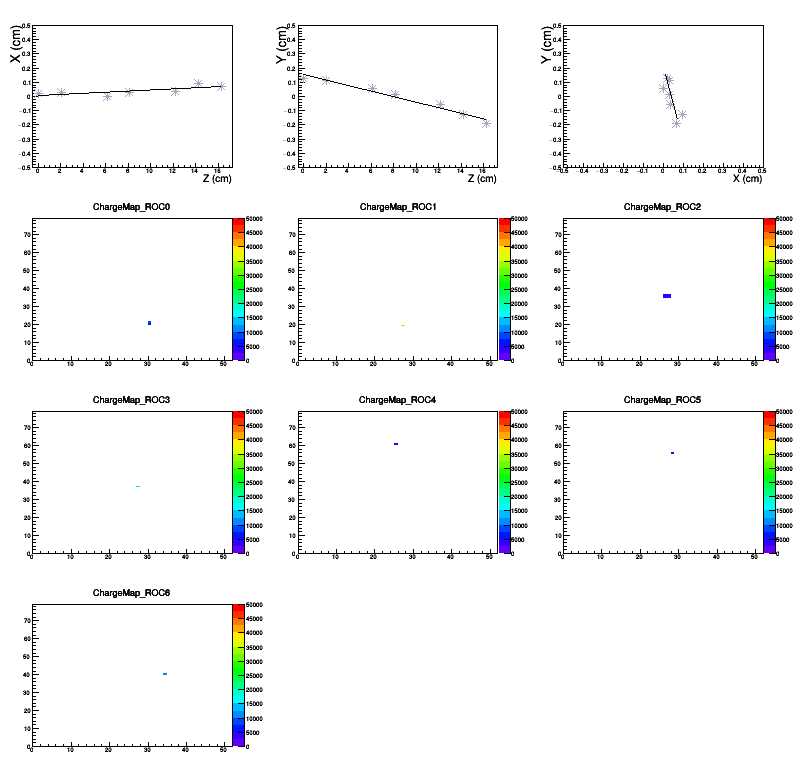
\includegraphics[width=5.5cm]{Pics/Tracks_Ev7}
		\end{minipage}\no\s
		\begin{itemize}
		\item display of random events of a run
	\end{itemize}
	\end{center}
\end{frame}
% ============================
% DOCUMENT END
\end{document}

